\documentclass{article}
\usepackage{graphicx} % Required for inserting images
\usepackage{amsmath} % For aligning equations
\usepackage{pgfplots} % For plotting graphs
\pgfplotsset{compat=1.18} % For pgfplots version 1.18 or later
\usepackage[colorlinks=true, linkcolor=blue, urlcolor=blue, citecolor=blue]{hyperref} % For hyperlinks

\begin{document}
% Do not forget to \usepackage{graphicx} in the main
\begin{titlepage}

    % Students preferences
    \title{Physics Homework 2}
    \author{Ivan Chabanov\\i.chananov@innopolis.university\\DSAI-03}

    % Image
    \begin{figure}[t]
        \centering
        
\includegraphics[width=0.69\textwidth]{innou-logo.png} % Adjust accordingly if renamed
    \end{figure}

    % Title itself
    \maketitle

\end{titlepage}
 % Include the title page


% Solution #1
\section*{Problem 1 Statement}
The figure shows the time dependence of velocity. Do the following:

\begin{enumerate}
    \item Plot the acceleration and displacement with respect to time. Assume the initial coordinate is $x(0) = 0$ m.
    \item Determine the displacement and the average velocity over the time interval $[t_1, t_3]$.
\end{enumerate}

Given: $t_1 = 4$ s, $t_2 = 10$ s, $t_3 = 18$ s.

\section*{Solution}

\subsection*{1. Acceleration and Displacement Plots}

\subsubsection*{Acceleration}
Acceleration is the change of the velocity over the time interval.
We have 3 time intervals: 
\[
t_0 = 0s, \quad t_1 = 4s, \quad t_2 = 10s, \quad t_3 = 18s.
\]
Velocity in these intervals:
\[
v_0 = 0 m/s, \quad v_1 = 4m/s, \quad v_2 = 4m/s, \quad v_3 = 0m/s.
\]
Knowing these variables, we can find the acceleration:

$$ a_1 = \frac{v_1 - v_0}{t_1 - t_0} = \frac{4 - 0}{4 - 0}m/s^2 = 1m/s^2  $$
$$ a_2 = \frac{v_2 - v_1}{t_2 - t_1} = \frac{4 - 4}{10 - 4}m/s^2  = 0m/s^2  $$ 
$$ a_3 = \frac{v_3 - v_2}{t_3 - t_2} = \frac{0 - 4}{18 - 10}m/s^2  = -0.5m/s^2  $$
So the acceleration is $a(t) = \begin{cases} 1 & 0 \leq t \leq 4 \\ 0 & 4 < t \leq 10 \\ -0.5 & 10 < t \leq 18 \end{cases}$.

\subsubsection*{Displacement}
We know, that the displacement is the change of the coordinate over the time interval. Coordinate formula:

% $$ x(t) = x(0) + v(0) \cdot t + a(t) \cdot \frac{t^2}{2} $$
\begin{equation}
    \label{eq:displacement}
    x(t) = x(0) + v(0) \cdot t + a(t) \cdot \frac{t^2}{2}
\end{equation}

As the point goes straight-line motion, the displacement could be found using the formula above.
Let us define a displacement over a time interval a:b as $ S_{[a:b]} $
Time calculation was omitted due to its simplicity.
$$ S_{[0:4]} = 0 + 0 \cdot t + 1 \cdot \frac{t^2}{2} = \frac{4^2}{2}m = 8m $$
$$ S_{[4:10]} = 8 + 4 \cdot t + 0 \cdot \frac{t^2}{2} = (8 + 4 \cdot 6)m = 32m $$
$$ S_{[10:18]} = 32 + 4 \cdot t - 0.5 \cdot \frac{t^2}{2} = (32 + 4 \cdot 8 - 0.5 \cdot \frac{8^2}{2})m = 48m $$
So the displacement is $S(t) = \begin{cases} 0 & t = 0 \\ 8 & t = 4 \\ 32 & t = 10 \\ 48 & t = 18 \end{cases}$.

\bigbreak Displacement graphs are a little bit trickier, that the acceleration ones.
In order to plot the displacement graph, let us clearly state coordinate function next using equation \ref{eq:displacement}.
We already got the coordinate functions over the intervals in the displacement section above, so let's use them.
Let us define the coordinate function on the interval a:b as $ x(t)_{[a:b]} $.
$$ x(t)_{[0:4]} = \frac{t^2}{2} $$
$$ x(t)_{[4:10]} = 4 \cdot t $$
$$ x(t)_{[10:18]} = 4 \cdot t - 0.5 \cdot \frac{t^2}{2} $$

But still we can not plot the graph using this functions as we have to transfer time in the future for some of them.
For example, $x(t)_{[4:10]}$ should be $x(t-4)_{[4:10]}$ as the body started to move this way only from 4th second.
Let us correct the functions:
$$ x(t)_{[0:4]} = \frac{(t-0)^2}{2} $$
$$ x(t)_{[4:10]} = 4 \cdot (t-4) $$
$$ x(t)_{[10:18]} = 4 \cdot (t-10) - 0.5 \cdot \frac{(t-10)^2}{2} $$
\bigbreak \centering \textit{Now we are ready for the graph plotting.}

\newpage \subsubsection*{Graph Plotting}
\begin{figure}[h!]
    \centering
    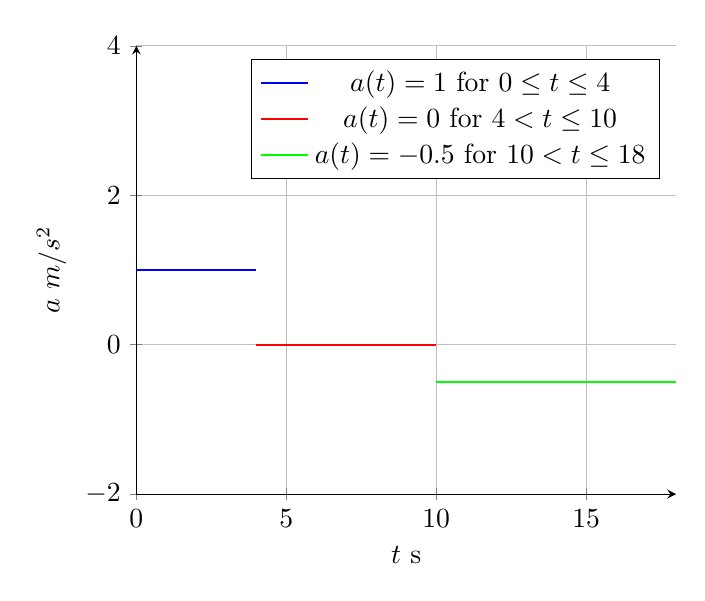
\begin{tikzpicture}
        \begin{axis}[
            axis lines = left,
            xlabel = $t$ s,
            ylabel = {$a$ ${m/s^2}$},
            ymin=-2, ymax=4,
            xmin=0, xmax=18,
            legend pos=north east,
            samples=100,
            grid=major,
        ]

        % Plot for the first interval: a(t) = 1 for 0 <= t <= 4
        \addplot[
            domain=0:4, 
            thick, 
            blue
        ] {1};
        \addlegendentry{$a(t) = 1$ for $0 \leq t \leq 4$}

        % Plot for the second interval: a(t) = 0 for 4 < t <= 10
        \addplot[
            domain=4:10, 
            thick, 
            red
        ] {0};
        \addlegendentry{$a(t) = 0$ for $4 < t \leq 10$}

        % Plot for the third interval: a(t) = -0.5 for 10 < t <= 18
        \addplot[
            domain=10:18, 
            thick, 
            green
        ] {-0.5};
        \addlegendentry{$a(t) = -0.5$ for $10 < t \leq 18$}

        \end{axis}
    \end{tikzpicture}
    \caption{Acceleration Plot}
    \label{fig:acceleration}

\end{figure}

\bigbreak \begin{figure}[h!]
    \centering
    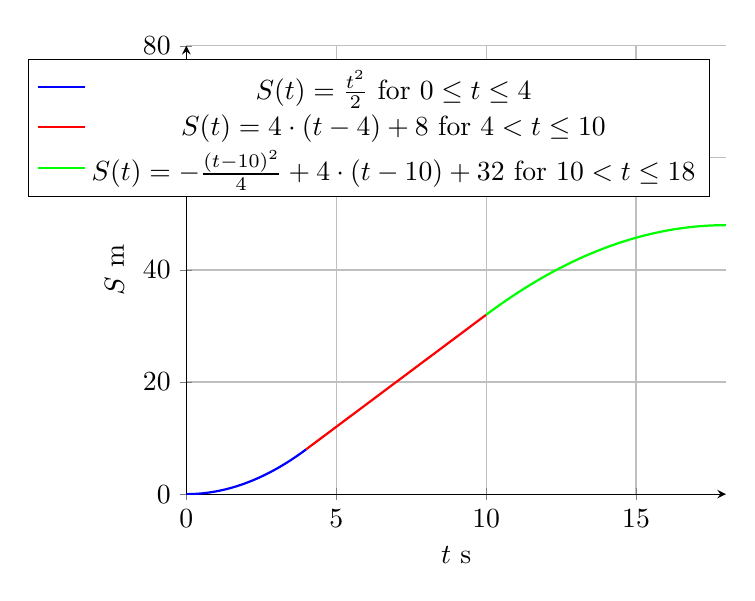
\begin{tikzpicture}
        \begin{axis}[
            axis lines = left,
            xlabel = $t$ s,
            ylabel = $S$ m,
            ymin=0, ymax=80,
            xmin=0, xmax=18,
            legend pos=north east,
            samples=100,
            grid=major,
        ]

        % Plot for the first interval: S(t) = t^2/2 for 0 <= t <= 4
        \addplot[
            domain=0:4, 
            thick, 
            blue
        ] {x^2/2};
        \addlegendentry{$S(t) = \frac{t^2}{2}$ for $0 \leq t \leq 4$}

        % Plot for the second interval: S(t) = 4(t-4) + 8 for 4 < t <= 10
        \addplot[
            domain=4:10, 
            thick, 
            red
        ] {4 * (x-4) + 8};
        \addlegendentry{$S(t) = 4 \cdot (t - 4) + 8 $ for $4 < t \leq 10$}

        % Plot for the third interval: S(t) = -(t-10)^2/4 + 4(t-10) + 32 for 10 < t <= 18
        \addplot[
            domain=10:18, 
            thick, 
            green
        ] {32 + 4*(x-10) - (x-10)^2/4};
        \addlegendentry{$S(t) = - \frac{(t - 10)^2}{4} + 4 \cdot (t - 10) + 32 $ for $10 < t \leq 18$}

        \end{axis}
    \end{tikzpicture}
    \caption{Displacement Plot}
    \label{fig:displacement}
\end{figure}

\raggedright \newpage \subsection*{2. Displacement and Average Velocity}
\subsubsection*{Displacement}
To find the displacement over the interval $[t_1, t_3]$ we take displacement over $[t_0, t_3]$ and subtract displacement over $[t_0, t_1]$.
This method will work as the movement is straight-line.

$$ S_{[t_1: t_3]} = S_{[t_0: t_3]} - S_{[t_0: t_1]} = S_{[0: 18]} - S_{[0: 4]} = (48 - 8)m = 40m $$

\subsubsection*{Average Velocity}
To find the average velocity over the interval $[t_1, t_3]$ we take displacement over $[t_1, t_3]$ and divide it by the time duration.

$$ v_{av[t_1: t_3]} = \frac{S_{[t_1: t_3]}}{t_3 - t_1} = \frac{40m}{(18 - 4)s} \approx 2.86m/s $$


\vfill % Pushes the following content to the bottom of the page

\subsection*{ANSWER}

\begin{enumerate}
    \item \hyperlink{fig:acceleration}{\ref*{fig:accelerationAcceleration} and \hyperlink{fig:displacement}{Displacement} plots.
    \item The displacement is $S = 40 m$.
\end{enumerate}

\end{document}